\documentclass{stdlocal}
\begin{document}
\section{Design and Implementation} % (fold)
\label{sec:design}

Experimenting with various designs and implementations of algorithms, that robustly and efficiently smooth discrete curves on surface meshes, requires to use a whole program pipeline or framework for loading input data, intuitively working with user interaction, and visualizing any intermediate results.
Unfortunately, providing a code base for such a framework in the appendix or the following subsections is out of the scope of this thesis.
Instead, all the following C++ code snippets represent simplified versions of program parts and do not strive for the best API design or implementation but rather a concise illustration on how to implement the provided data structures and primitives.
% As changing specific parts of such a pipeline may affect the performance, outcomes, and overall behavior of an algorithm or program, a brief overview over all of its components is essential to allow for reproducible results and will therefore be given in the following subsections.
% This will also make it possible for readers to simply reconstruct, adjust, and improve the pipeline for their own domain-specific projects.
% Afterwards, I will thoroughly elaborate on the design and implementation of chosen data structures and algorithms together with their mathematical primitives for curve smoothing.

% The pipeline or framework, described in this thesis, has been manually implemented with the C++ programming language and the OpenGL graphics API using some external libraries to handle low-level tasks.
% Already described in the introduction in section~\ref{sec:introduction}, this choice is well suited for open-source graphics applications and provides programmers with a large freedom when it comes to the implementation of data structures and algorithms.
% The complete source code of the project, called \textit{nanoreflex}, is provided as an open-source repository on GitHub.

\subsection{Data Structures for Polyhedral Surfaces} % (fold)
\label{sub:polyhedral_surface_data_structure}

  In general, the choice and efficiency of algorithms highly depends on underlying data structures that represent the intermediate data of a program \autocite{knuth1997,mehlhorn2008,smed2006}.
  Thus, thorough design considerations for the data structures of polyhedral surfaces and surface mesh curves are mandatory to build fast and robust curve smoothing algorithms.
  Regarding the context of this thesis, I will focus on orientable polyhedral surfaces.
  As it was already explained before, this is not an actual restriction for the algorithm but will only speed up the implementation.
  Typical surfaces are the boundary of volumes that can be viewed as 3D open submanifolds of the 3D Euclidean space.
  These volumes must be oriented by construction and, hence, the boundary which represents the surface is oriented, too.

  To be able to render a triangular surface mesh in OpenGL, a simple and versatile method is to provide two separate lists for vertices and triangles, respectively \autocite{opengl}.
  Hereby, each triangle only references its three vertices by using indices that may be used to extract a vertex from the vertex list.
  The orientation of a triangle is defined by the order of its vertex references based on the description given in section~\ref{sec:preliminaries} in the preliminaries.
  Furthermore, vertices in OpenGL are quite general and may not only store their own positions.
  Typically, attributes for pseudo-normals, colors, or texture coordinates are added to use sophisticated shading techniques and improve the quality of illustrations.
  A concrete implementation of this can be seen in the following code snippet.
  Additionally, figure~\ref{fig:polyhedral-surface-faces} shows an example to visualize the memory layout of the vertex and face list.

  \begin{figure}[b]
    \centering
    \begin{subfigure}[c]{0.35\linewidth}
      \centering
      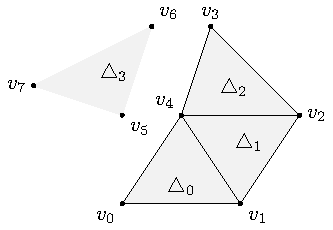
\includegraphics[width=\linewidth]{figures/polyhedral-surface-struct-base-scheme.pdf}
    \end{subfigure}
    \hfill
    \begin{subfigure}[c]{0.63\linewidth}
      \centering
      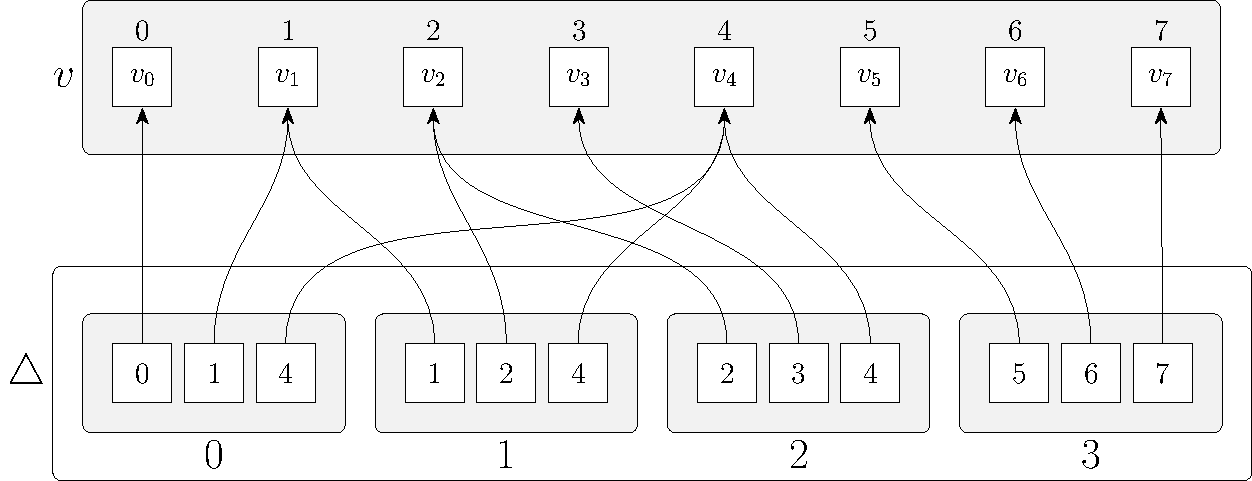
\includegraphics[width=\linewidth]{figures/polyhedral-surface-struct-base.pdf}
    \end{subfigure}
    \caption[Data Structure for Faces of a Polyhedral Surface]{%
      \textbf{Data Structure for Faces of a Polyhedral Surface}\\
      The figure shows a schematic example of how faces of a given polyhedral surface (left) are stored in memory.
      The surface consists of eight enumerated vertices and four faces.
      As it can be seen on the right, each face references three distinct vertices by their index in the order of their orientation.
      This way one vertex can be used by multiple triangles.
    }
    \label{fig:polyhedral-surface-faces}
  \end{figure}

  \inputCodeBlock[title = Vertices and Faces]{code/vertices-and-faces.hpp}

  \noindent
  As polyhedral surfaces are a special form of 3D surface geometry, I will use file formats, such as STL \autocite{stl-file-format} and Wavefront OBJ \autocite{obj-file-format}, to provide the possibility for reading complex surface meshes from disk.
  Especially in the area of computer graphics in conjunction with the C++ programming language, the \textit{Assimp} library \autocite{assimp} is often used to load even more file formats that represent general surfaces and scenes.
  The facility makes it possible to test algorithms with very complex surface meshes from the \citetitle{thingi10k} dataset whose models are mainly provided as STL files.

  This representation already allows for an OpenGL-based visualization of polyhedral surfaces with sufficient quality by adding GLSL shaders.
  But in the context of this thesis, also the efficient movement of points and curves along the surface mesh needs to be possible.
  Over and over trying to determine adjacent neighbors of vertices or triangles with this data structure quickly becomes infeasible.
  So, further surface mesh preprocessing steps are needed to generate and store essential adjacency information.

  Computing and storing neighbor and adjacency information of surface meshes is a studied and vast area of computational geometry.
  There are multiple well-known data structures, like Quad-Edge Algebras \autocite{guibas1985} and triangular adjacencies \autocite{shewchuk1996}, for handling graphs that represent the topological structure of general 2D polyhedral surfaces.
  These data structures have successfully been used to efficiently construct Delaunay triangulations and encode the information of 3D surface meshes.
  The quad-edge algebra, described by \textcite{guibas1985}, is a versatile and complex data structure based on edges that represents both, the graph and the dual graph, of the surface at once and allows to easily and efficiently access the lists of adjacent vertices, edges, and faces.
  A simple but efficient implementation that does not make use of any pointers is given in section~\ref{sec:quad_edge_algebra} in the appendix.
  Figure~\ref{fig:quad-edge} and \ref{fig:quad-edge-rotation} schematically show the memory layout and rotation primitive of the data structure.

  On the other hand, according to \textcite{shewchuk1996}, a flat adjacency list storing references to adjacent faces for each face offers a lower memory consumption and an expected efficiency higher than that of a quad-edge algebra at the cost of a higher programming complexity when used in algorithms.
  It does not provide an easy way to access the graph but still incorporates the dual graph of the surface and is much easier to generate and handle than the quad-edge algebra.
  As each triangle may at most exhibit three other triangles that are adjacent to it, there is an upper storage bound for adjacency references of each triangle.
  Triangular adjacencies already have been used by \textcite{mancinelli2022} to implement one of the fastest geodesics tracing algorithms.
  Still, the adjacencies itself make it hard to access the circular list of adjacent faces around a vertex.
  My solution for triangular adjacencies, that will be explained in the following, uses insights gained from the quad-edge algebra and slightly changes the standard face references by adding locations to cope with this disadvantage.

  Unfortunately, the connectivity information provided by the faces and vertices are not suitable for surface mesh curves and smoothing algorithms.
  In an OpenGL-based rendering pipeline, the vertices of a polyhedral surface must differ as soon as they exhibit at least one distinct attribute.
  Even though triangles could share the same vertex position, their respective vertices might contain different pseudo-normals to model a crease in the surface and, consequently, these triangles cannot reference the same vertex.
  Even worse, for various reasons, it is allowed to use multiple instances of the same vertex inside the vertex list which also would lead to distinct vertex references.
  Especially, in the extreme case of STL files, every triangle uniquely refers to vertices that cannot be referred by other triangles which is schematically visualized in figure~\ref{fig:polyhedral-surface-distinct-vertices}.
  On the other hand, the values for additional attributes of a vertex, like pseudo-normals or texture coordinates, are unimportant for algorithms handling surface mesh curves and may be neglected as they do not change the topology of the underlying polyhedral surface.
  Such an algorithm would need to assume two vertices to be equivalent as long as they exhibit the same position.
  As a consequence, naively generating the graph or dual graph of the surface mesh solely based on the vertices and faces will not result in the correct topological connectivity needed for surface mesh curves.

  \begin{figure}[t]
    \centering
    \begin{subfigure}[c]{0.40\linewidth}
      \centering
      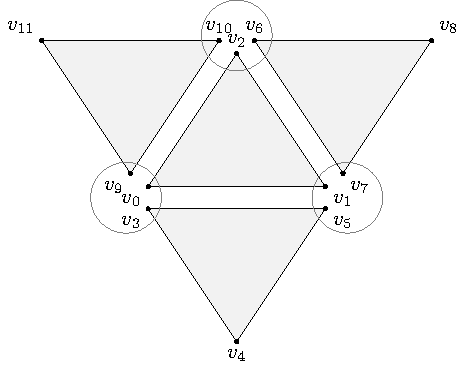
\includegraphics[width=\linewidth]{figures/polyhedral-surface-separated.pdf}
    \end{subfigure}
    \hfill
    $\longrightarrow$
    \hfill
    \begin{subfigure}[c]{0.40\linewidth}
      \centering
      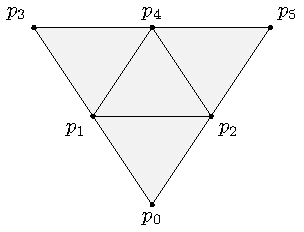
\includegraphics[width=\linewidth]{figures/polyhedral-surface-joint.pdf}
    \end{subfigure}
    \caption[Connectivity by Using Topological Vertices]{%
      \textbf{Connectivity by Using Topological Vertices}\\
      On the right, a simple polyhedral surface with six topological vertices and four faces is shown.
      In a data structure suitable for OpenGL-based rendering, each triangle might reference its own unique vertices as shown on the left.
      These vertices are distinct from each other which logically disconnects the four adjacent triangles.
    }
    \label{fig:polyhedral-surface-distinct-vertices}
  \end{figure}

  The use of surface mesh curves and smoothing algorithms should neither put a higher burden on the OpenGL pipeline nor require dramatic changes to data structures used for rendering.
  My solution to that problem generates an additional topological structure that extends the connectivity information given by the basic structure.
  Hereby, the main idea was that the projection of vertices onto their positions can be modeled by the quotient space and its respective quotient map.
  In this sense, let $\mathscr{V}$ be the set of all vertices and $\function{p}{\mathscr{V}}{\setReal^3}$ be the function that maps a vertex to its position in space.
  Two vertices $v,w\in\mathscr{V}$ are called to be topologically equivalent, denoted as $v\sim w$, if they exhibit the same position.
  \[
    v \sim w
    \quad :\iff\quad
    p(v) = p(w)
  \]
  Then the quotient space $\mathscr{V}/\sim$ consists of equivalence classes whose elements are pairwise topologically equivalent vertices.
  These equivalence classes will from now on be called topological vertices.
  The respective quotient map τ of $\mathscr{V}/\sim$ is given as follows.
  \[
    \function{τ}{\mathscr{V}}{\mathscr{V}/\sim}
    \separate
    τ(v) \define [v]
  \]

  \begin{figure}
    \centering
    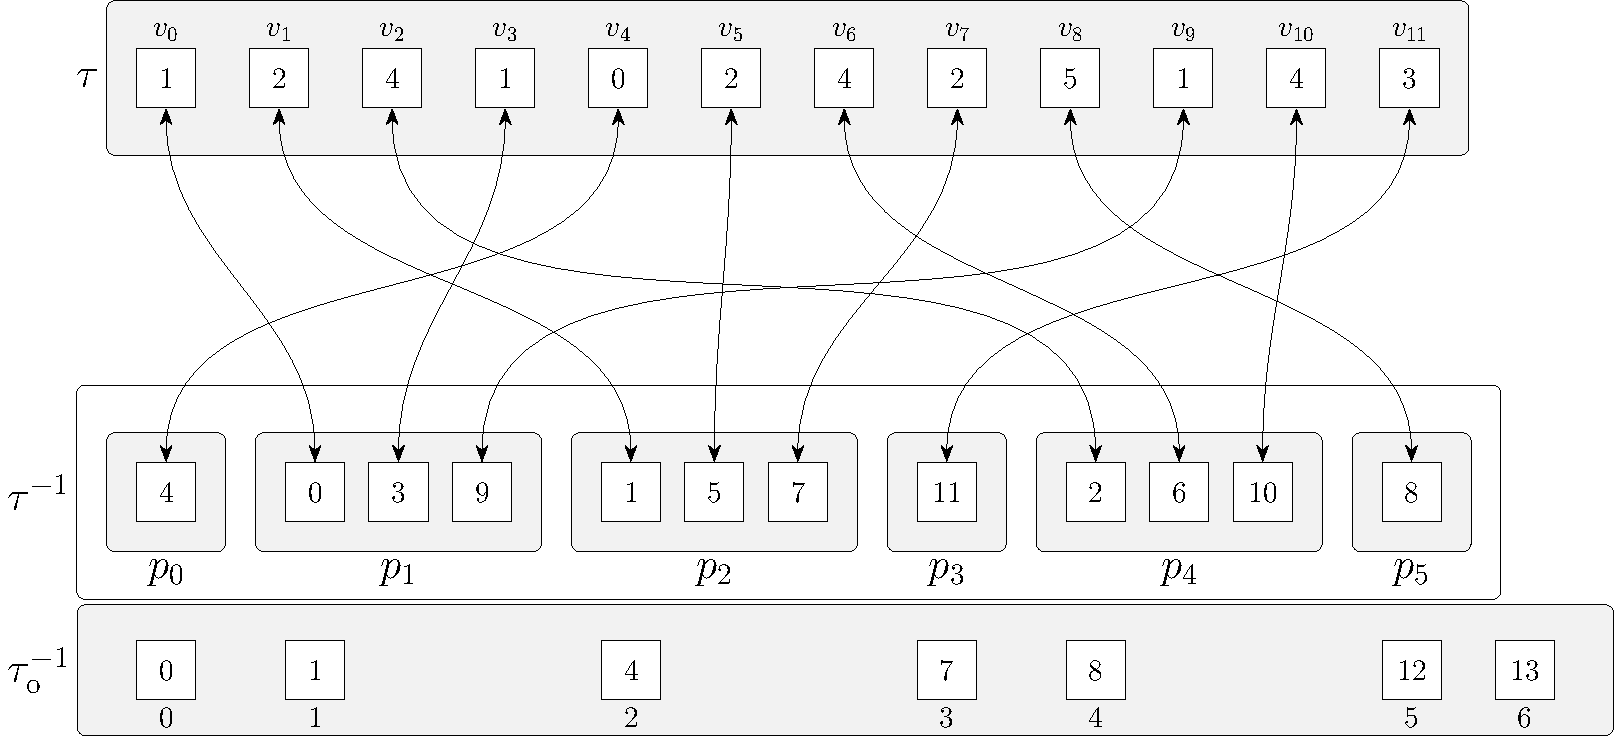
\includegraphics[width=\linewidth]{figures/polyhedral-surface-topological-vertex-map.pdf}
    \caption[Topological Quotient Map]{%
      \textbf{Topological Quotient Map}\\
      The figure schematically shows the quotient map τ of the polyhedral surface given in figure~\ref{fig:polyhedral-surface-distinct-vertices} which maps vertices onto their topological counterparts.
      As this map is not bijective, its inverse $τ^{-1}$ must use another array $τ^{-1}_\mathrm{o}$ of offsets.
    }
    \label{fig:polyhedral-surface-topological-vertex-map}
  \end{figure}

  \noindent
  Two triangles are topologically adjacent to each other if they share a topological edge and are not identical.
  Using the quotient map, a rigorous formulation can be given as follows.
  Let $n\in\setNatural$ be the number of vertices in the vertex list $\function{V}{\mathscr{I}}{\mathscr{V}}$ with $\mathscr{I}\define\set{k\in\setNatural_0}{k\leq n}$ as the index set.
  Two triangles of the faces list given by index triples $(v_1,v_2,v_3)$ and $(w_1,w_2,w_3)$ are adjacent to each other if there are permutations $σ,π\in\mathrm{S}_3$ such that the following holds.
  \[
    τ(V(v_{σ(1)})) = τ(V(w_{π(1)}))
    \separate
    τ(V(v_{σ(2)})) = τ(V(w_{π(2)}))
  \]
  \[
    τ(V(v_{σ(3)})) \neq τ(V(w_{π(3)}))
  \]
  Hence, by constructing the quotient map τ, I will be able to correctly determine topological connections.
  Still, the naive evaluation of the topological equivalence relation $\sim$ for all vertices is quadratic in complexity.
  For high-resolution polyhedral surfaces with millions of triangles, this is infeasible and needs to be addressed.

  For this, my solution is based on a hash map in which all vertices will be inserted with respect to their position in space.
  As 3D vectors do not provide a natural order, a custom hash function needs to be used.
  Furthermore, the standard equality comparison is exchanged with the topological equivalence relation.
  This way topologically equivalent vertices are assumed to be the same by the hash map and are inserted at identical positions.
  Each insertion has an expected constant-time complexity.
  As a result, the insertion of all vertices exhibits a linear time complexity and offers a more efficient alternative to the naive method of checking pairwise equivalences.
  The following code snippet demonstrates a simple implementation of this method in C++.
  Additionally, figure~\ref{fig:polyhedral-surface-topological-vertex-map} schematically visualizes how the quotient map for the example given in figure~\ref{fig:polyhedral-surface-distinct-vertices} would look.

  \inputCodeBlock[title = Topological Vertex Map]{code/topological-vertex-map.hpp}

  \noindent
  With the above implementation, the inverse of the quotient map cannot directly be evaluated.
  This is a major drawback when working with edge-based data structures as these must reference topological vertices and there would be no efficient way to determine their position or shared pseudo-normals.
  If it is sufficient to access the positions of topological vertices then a simple copy of the positions might be the best way.
  In all other cases, the following code snippet provides a way to construct the inverse of the quotient map.
  Again, figure~\ref{fig:polyhedral-surface-topological-vertex-map} visualizes the inverse of the example given in figure~\ref{fig:polyhedral-surface-distinct-vertices}.
  As the quotient map is not bijective, an additional offset array is used to get the list of all vertices that refer to the same topological vertex.

  \inputCodeBlock[title = Inverse Topological Vertex Map]{code/inverse-topological-vertex-map.hpp}
  First, the code snippet calculates the cardinality of the equivalence classes representing topological vertices.
  Then by iteratively building the cumulative sum of cardinalities the data offset for each topological vertex has been determined.
  This offset is then used to add backwards pointing vertex references to the inverse map.
  As the offsets are changed by this operation, a final step shifts all the offsets to the left to repair the offset array.
  Getting all the vertex references of a topological vertex then only means to iterate over indices starting at the respective offset and ending before the next offset.

  With the availability of topological vertices and their correspondence to vertices, the next important intermediate construction step is the generation of all surface edges.
  During this construction step the given surface can be checked for orientability and consistency.
  Hereby, consistency means whether or not the vertices and faces fulfill the requirements of a 2D topological manifold.
  Furthermore, the intermediate representation of edges given below allows to determine nearly all the adjacency structures for vertices, edges, and faces.
  For this, a hash map of directed edges with a custom hash function for edges will be constructed by iterating over the list of faces.
  Hereby, each face will interpreted as an oriented triangle that adds all of its three directed edges to the hash map.
  The values for each directed edge in the hash map will refer to its specific triangle and its location inside that triangle.

  \inputCodeBlock[title = Intermediate Topological Edges]{code/topological-directed-edges.hpp}
  At the start of the code snippet, structures for face adjacency references and directed edges are defined to simplify the implementation of edge generation.
  Directed edges are simply represented by two references to topological vertices.
  As they need to be added to a hash map, an information structure and a hash function have been added.
  The information structure only stores two face adjacencies to let the directed edge know from which face and at which location it originated.
  A face adjacency reference refers to a face in the face list and additionally to the edge location inside that face at which the adjacency occurs.
  As there are only three possible locations, only two bits are used to encode this information in the standard face reference by using the bit-field feature of C++.
  This reduces the amount of referencable faces to $2^{30}$ which is a little over 1~billion triangles.
  The memory consumption for this case would be $36\appendUnit{GiB}$ at minimum for the vertex and face list implementations provided here.
  Even nowadays graphics cards customary in trade are not able to handle this huge amount of data at once.
  Hence, the implementation does not impose serious constraints on the data it can handle.

  Now, to generate the topological face adjacencies, all that is to do is to iterate over all edges and add their mapped information to the face adjacencies.
  In the case that a triangle is part of the boundary of the polyhedral surface, a non-existing neighbor is marked as an invalid reference.
  The following code snippet demonstrates this.
  In figure~\ref{fig:polyhedral-surface-face-adjacencies}, a scheme that visualizes the memory layout of the topological face adjacencies can be seen.

  \begin{figure}
    \centering
    \begin{subfigure}[c]{0.38\linewidth}
      \centering
      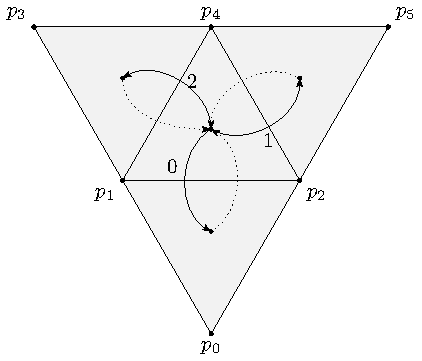
\includegraphics[width=\linewidth]{figures/polyhedral-surface-triangle-adjacencies.pdf}
    \end{subfigure}
    \hfill
    \begin{subfigure}[c]{0.60\linewidth}
      \centering
      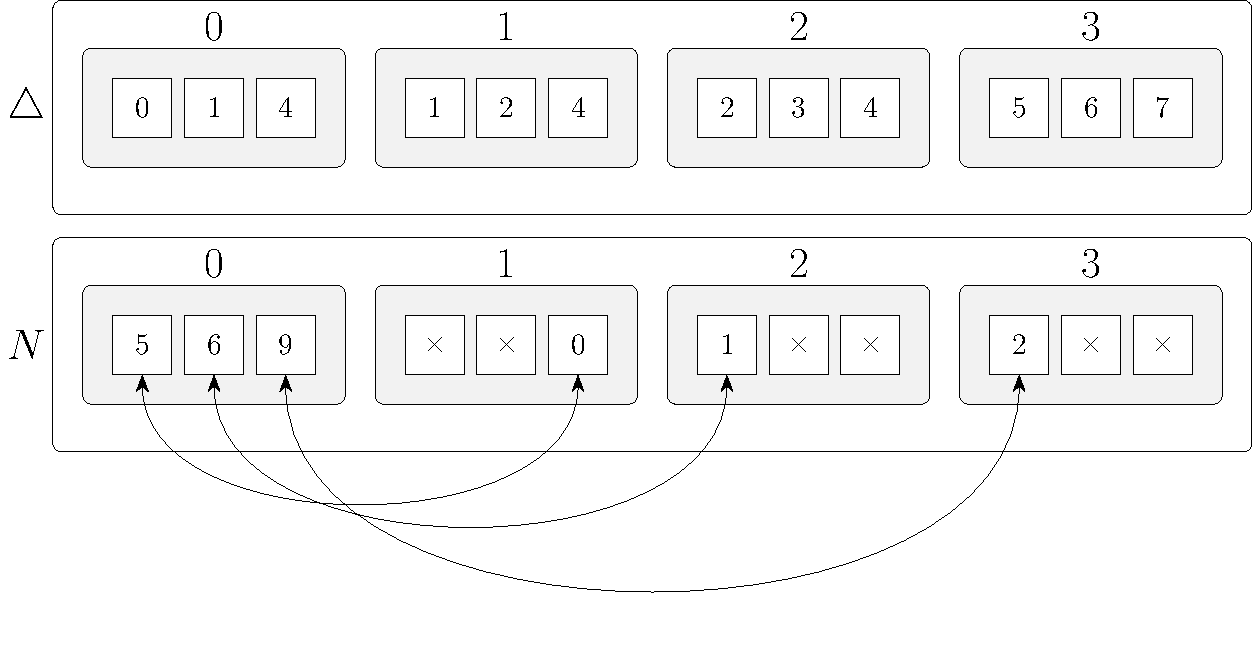
\includegraphics[width=\linewidth]{figures/polyhedral-surface-triangle-adjacencies-struct.pdf}
    \end{subfigure}
    \caption[Topological Face Adjacencies]{
      \textbf{Topological Face Adjacencies}\\
      The figure schematically visualizes how face adjacencies are stored in memory.
      On the left, the inner face of the polyhedral surface is surrounded by three other faces.
      For all these faces, its adjacency structure provides the face reference and the location inside their adjacency structure that points back to the inner face.
      In this example, the face adjacency is given by $N = 3f + l$ with $f$ as the face reference and $l$ as the location.
      Please note, in the code provided in this section, instead $N = 4f + l$ in the form of a bit-field is used for efficiency reasons.
    }
    \label{fig:polyhedral-surface-face-adjacencies}
  \end{figure}

  \inputCodeBlock[title = Topological Face Adjacencies]{code/topological-face-adjacencies.hpp}
  During the iteration over all directed edges, the code snippet distinguishes between oriented and unoriented edges.
  In the case of an oriented edge, the information structure only provides one valid face adjacency reference.
  Thus, the hash map of edges is queried for the reverse edge to get its information structure and with it the reference to the adjacent face.
  If the reverse edge does not exist, the current edge must be part of the boundary.

  Incorporating the location values into face adjacencies allows for an easy navigation along oriented polyhedral surfaces.
  Figure~\ref{fig:polyhedral-surface-face-adjacency-rotation} shows the basic operation for face adjacencies that rotates the current direction of the adjacency counterclockwise similar to quad-edge rotations of figure~\ref{fig:quad-edge-rotation}.
  It can be implemented by adding $1$ to the location and afterwards taking its modulus base $3$.
  This primitive enables the code to easily run through the list of triangles around a vertex in clockwise and counterclockwise order.
  Furthermore, for an algorithm which makes only use of the flat list of face adjacencies, the quotient map for topological vertices and the hash map for directed edges can be destroyed.
  In fact, the topological face adjacencies have been generated by the use of topological vertices but their data do not reference these anymore.

  \begin{figure}
    \centering
    \begin{subfigure}[c]{0.31\linewidth}
      \centering
      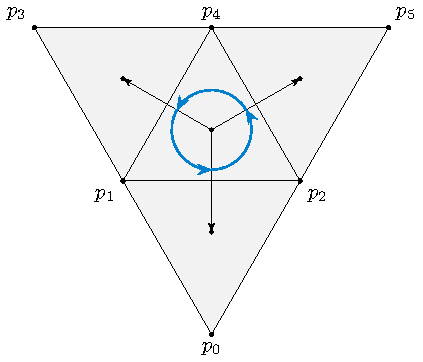
\includegraphics[width=\linewidth]{figures/polyhedral-surface-triangle-adjacencies-rot.pdf}
    \end{subfigure}
    \hfill
    \begin{subfigure}[c]{0.67\linewidth}
      \centering
      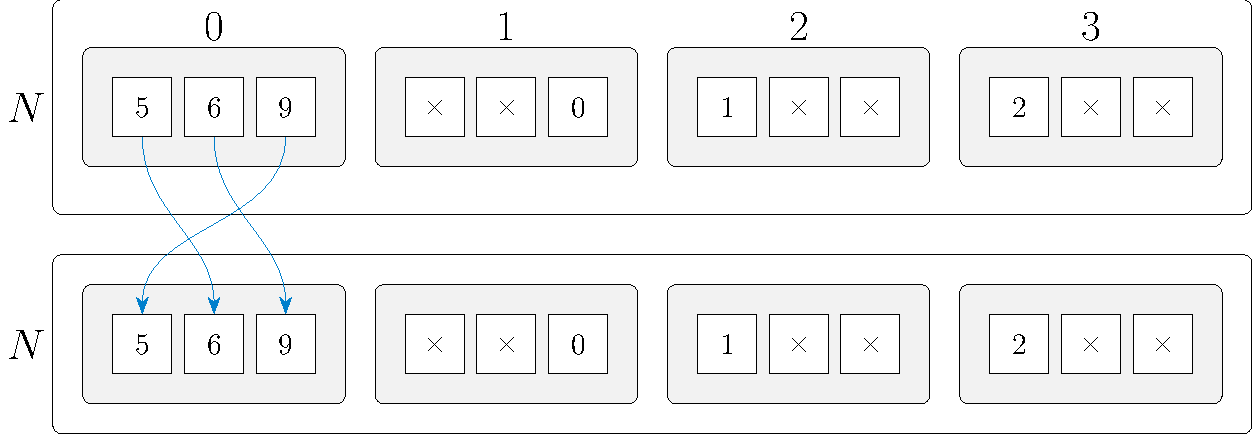
\includegraphics[width=\linewidth]{figures/polyhedral-surface-triangle-adjacencies-rot-struct.pdf}
    \end{subfigure}
    \caption[Counterclockwise Rotation of Topological Face Adjacencies]{
      \textbf{Counterclockwise Rotation of Topological Face Adjacencies}\\
      The rotation of face adjacencies (shown in blue) can be implemented by adding $1$ to the location and then taking its modulus base $3$.
      Using this operation together with all the face adjacencies allows to iterate through the list of faces around a vertex in clockwise and counterclockwise order.
    }
    \label{fig:polyhedral-surface-face-adjacency-rotation}
  \end{figure}

  As already described in section~\ref{sec:preliminaries} in the preliminaries, the vertices and edges of a polyhedral surface model a vertex-based graph which characterizes the vertex adjacencies.
  Looking at a polyhedral surface in this way, storing the triangle adjacencies makes the corresponding dual graph available.
  For the vertex-based graph, the adjacent vertices of each vertex would need be determined first.
  An efficient structure to store vertex neighbors is a sparse matrix in the compressed sparse row format without an extra array for matrix entries.
  The construction of counterclockwise oriented neighbor entries can be done by using the face adjacencies.
  Still, the boundary of a surface mesh needs to be handled by additional facilities as the vertex-based graph structure itself does not exhibit a way to simply encode them.
  Furthermore, the vertex-based graph needs to reference topological vertices and each vertex might have arbitrary many neighbors.

% subsection polyhedral_surface_data_structure (end)

\subsection{Data Structures for Surface Mesh Curves} % (fold)
\label{sub:discrete_surface_curve_data_structure}

  The representation of surface mesh curves via data structures may follow two main approaches and depends on the choice of data structures used to store topological adjacency information of the underlying polyhedral surface.

  \paragraph{Edge-Based Data Structure}\hfill\\
  On the one hand, surface mesh curves can solely be characterized by a list of control points over the surface mesh of a polyhedral surface.
  As the surface mesh is the union of topological edges, a natural construction would be based on a list of edges that contain the control points of the curve, respectively.
  To specify their exact position, an additional weighting parameter would need to be provided for every edge.
  Furthermore, in essence, the smoothing process can also be described as the movement of the curve along the surface.
  So, a feature is needed to map specific information of the initially given curve onto successive evolutions of the curve smoothing process.
  The following code snippet shows a simple implementation of these ideas.

  \inputCodeBlock[title = Edge-Based Surface Mesh Curve]{code/surface-mesh-curve-edge-based.hpp}
  Presumably, the code snippet above describes one of the easiest possible data structures as it represents a surface mesh curve directly as a list of control points.
  Hereby, the simple edge structure uses references to topological vertices and its direction will always point to the right side of the curve on the surface.
  Closed curves can be represented by letting the last and the first point coincide.
  If the control point would need to represent a single vertex of the surface, both edge references should point to the same topological vertex.

  Unfortunately, this edge structure does not offer the ability to simply access adjacent edges or faces.
  Instead, all operations to change an edge and, as a consequence, the topology of the featured surface mesh curve are bound to either use the temporary hash map of directed edges or the adjacency structure for vertex neighbors in conjunction with a mask to identify boundary vertices.
  But using a sparse matrix of vertex neighbors, it is again possible to check for regularity of the surface mesh curve.
  In a regular surface mesh curve, three adjacent control points are not allowed to lie on the same triangle.
  For this, the edge of the next control point is not allowed to be the same as the edges of the current or previous control points.
  Additionally, it must also not be part of the edge that connects the edges of the previous and current control points.

  \paragraph{Face-Based Data Structure}\hfill\\
  On the other hand, face-based data structures have been successfully used before to implement surface mesh curves \autocite{mancinelli2022}.
  The idea is basically to not directly reference edges but instead use references to their two adjacent faces.
  Using this, not a list of edges with their weights is used but a strip of adjacent faces.
  Each pair of adjacent triangles represents their common edge that is used as the location of the control point.
  As before, separate lists of edge weights and mapping parameters that directly correspond to the common edges are needed.
  Figure~\ref{fig:surface-mesh-curve-face-based} explains this principle by a schematic example.

  \begin{figure}
    \centering
    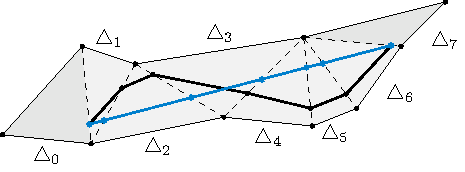
\includegraphics[width=0.8\linewidth]{figures/surface-mesh-curve.pdf}
    \caption[Face-Based Surface Mesh Curve]{%
      \textbf{Face-Based Surface Mesh Curve}\\
      The figure schematically shows an unfolded strip of adjacent triangles that are part of a polyhedral surface.
      Additionally, two surface mesh curves in black an blue are shown.
      Their control points are part of the edges of each pair of adjacent triangles.
      The blue surface mesh curve is also a discrete geodesic.
    }
    \label{fig:surface-mesh-curve-face-based}
  \end{figure}


  A strip of adjacent triangles only needs to access the flat list of face adjacencies and can get rid of additional boundary information or references to topological vertices.
  However, a face-based data structure for surface mesh curves does not come without problems, that are mostly overlooked in the literature \autocite{mancinelli2022}, but that still need to be addressed.

  First, to get the common edge of two adjacent triangles by only using simple face references is a tedious task since every neighbor reference of a triangle would need to be checked.
  This is a process that needs to be done many times for each iteration and as such would result in a large inefficiency.

  Second, a face-based representation is not applicable to general surface mesh curves.
  For this, refer to the left part of figure~\ref{fig:surface-mesh-curves-face-based-regularization}.
  Representing control points by positions on the common edges of adjacent faces induces some regularity conditions on the curve.
  Indeed, this is not too much of a problem as all further primitives will only deal with regular surface mesh curves whose topology is always representable by a strip of adjacent faces.

  \begin{figure}
    \centering
    \begin{subfigure}[c]{0.38\linewidth}
      \centering
      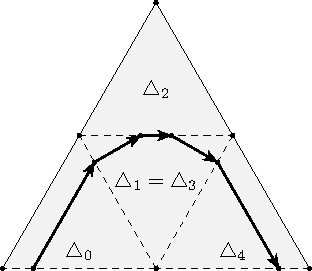
\includegraphics[width=\linewidth]{figures/surface-mesh-curve-artifact.pdf}
    \end{subfigure}
    $\quad\longrightarrow\quad$
    \begin{subfigure}[c]{0.38\linewidth}
      \centering
      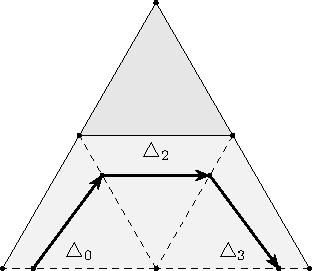
\includegraphics[width=\linewidth]{figures/surface-mesh-curve-artifact-removed.pdf}
    \end{subfigure}
    \caption[Regularization of Irregular Triangle Paths]{
      \textbf{Regularization of Irregular Triangle Paths}\\
      Using a face-based data structure to represent surface mesh curves already imposes some regularity conditions.
      As can be seen on the left side, irregular surface mesh curves still might originate when the next triangle in the face strip coincides with the previous one.
      The regularization transformation removes $\triangle_1$ and $\triangle_2$ as soon as $\triangle_3$ is added.
      The result can be seen on the right side.
    }
    \label{fig:surface-mesh-curves-face-based-regularization}
  \end{figure}

  Third, open surface mesh curves may provide start and end points on edges that are part of the boundary of the polyhedral surface.
  Boundary edges do not have two adjacent faces that could represent their common edge.
  To allow face-based curves to represent curves that start or end on boundaries, one could use the idea proposed by \textcite{shewchuk1996} to add so-called phantom triangles to each boundary edge that will not be rendered and are only used virtually.
  In figure~\ref{fig:surface-mesh-curve-face-based}, these phantom triangles would correspond to the triangles $\triangle_0$ and $\triangle_7$ which are marked by a darker gray.

  My face-based data structure for regular surface mesh curves on the other hand does not use phantom triangles and slightly changes the basic idea of a face strip.
  Thinking of a doubly linked list, I let the face references of the strip also provide the locations to the previous and next virtual triangles.
  In such a way, the faces represent the previous and next edge at the same time.
  For consistency, the next edge of a given face in the strip must coincide with the previous edge of the next adjacent face.
  In the case of boundary edges, it is clear from the observations of section~\ref{sec:preliminaries} about the mathematical preliminaries, that boundary edges apart from their vertices are only allowed to contain the first or last control point of a regular surface mesh curve.
  Therefore start and end points on a boundary edge can be represented by the previous and next location of the first and last triangle in the strip, respectively.
  Regarding the example given in figure~\ref{fig:surface-mesh-curve-face-based}, the face strip in this context would remove the triangles $\triangle_0$ and $\triangle_7$ and be given by $(\triangle_1,\triangle_2,\triangle_3,\triangle_4,\triangle_5,\triangle_6)$.
  The following code snippet provides a simple implementation of this data structure.

  \inputCodeBlock[title = Face-Based Surface Mesh Curve]{code/surface-mesh-curve-face-based.hpp}
  It has already been figured out that using a face-based data structure, requires the implementation to separate the edge weights from the triangle strip.
  As described above, in addition to a face reference, each face-based node in the code stores the location of its adjacency that points to the previous face and encodes the location to the adjacency that points to the next face.
  Hereby, the location for the next face is given by its difference to the subsequent location for the previous face.
  This encoding has been chosen because it can also be represented by a single bit and models the question whether the next edge of the current face turns to the left.
  Figure~\ref{fig:surface-mesh-curve-turns} shows the idea behind right and left turns.
  The difference between the previous and the next location inside a face node is either $1$ when the next edge turns to right or $2$ when the next edge turns to the left.
  As surface mesh curves do use essentially less points than polyhedral surfaces, it is not needed to encode the location information into the face reference itself.
  For the representation of closed surface mesh curves by the given face-based data structure only the last face's next location would need to point to the first face in the strip and the first face's previous location to the last face in the strip.
  This way each edge would consistently be referenced twice inside the face strip.
  For the edge weights, the same procedure as before is used.
  The first parameter is copied to the end of the edge weight list.
  Also the check for regular surface mesh curves is simplified.
  One only needs to check that the next face in the strip is not the same as the current or previous face.
  % The regularization of face-based surface mesh curves can be implemented in a much simpler way by making sure the next face is not the same as the previous or current face.

  \begin{figure}
    \centering
    \begin{subfigure}[b]{0.45\linewidth}
      \centering
      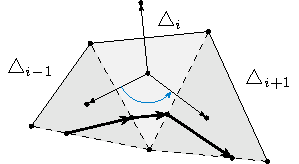
\includegraphics[width=\linewidth]{figures/surface-mesh-curve-rot-right.pdf}
      \caption{Right}
    \end{subfigure}
    \hfill
    \begin{subfigure}[b]{0.45\linewidth}
      \centering
      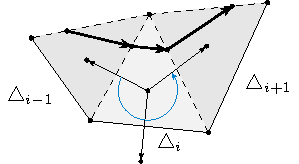
\includegraphics[width=\linewidth]{figures/surface-mesh-curve-rot-left.pdf}
      \caption{Left}
    \end{subfigure}
    \caption[Right and Left Turns of Face-Based Surface Mesh Curves]{
      \textbf{Right and Left Turns of Face-Based Surface Mesh Curves}\\
      Regarding the face strip of a regular surface mesh curve, for each face in the strip there are only two possible triangles that may follow as adjacent faces.
      For oriented polyhedral surfaces, these possibilities represent right and left turning of the next edge.
      In the case of a right turning edge, the difference of the previous and next location in triangle $\triangle_i$ is $1$ and $2$ for a left turning edge.
    }
    \label{fig:surface-mesh-curve-turns}
  \end{figure}

  \paragraph{Turn Compression}\hfill\\
  With the use of appropriate adjacency structures for a polyhedral surface, such as the flat face adjacency list, the underlying topology of a surface mesh curve can be represented in a compressed structure.
  Referring to figure~\ref{fig:surface-mesh-curve-turns}, this compression scheme contains the starting face adjacency and a list of right or left turns.
  % Additionally, the first face adjacency needs to be stored as a starting point.
  % Figure~\ref{fig:surface-mesh-curve-turns} schematically shows the idea behind the turn of a surface mesh curve.
  For the example given in figure~\ref{fig:surface-mesh-curve-face-based}, the turn scheme can be formulated in the two following ways.
  \[
    \textit{Right}
    \ \longrightarrow\
    \textit{Left}
    \ \longrightarrow\
    \textit{Right}
    \ \longrightarrow\
    \textit{Left}
    \ \longrightarrow\
    \textit{Left}
    \ \longrightarrow\
    \textit{Left}
  \]
  \[
    1\times\textit{Right}
    \ \longrightarrow\
    1\times\textit{Left}
    \ \longrightarrow\
    1\times\textit{Right}
    \ \longrightarrow\
    3\times\textit{Left}
  \]
  The turn scheme in its first formulation is already part of my face-based data structure and encoded in each face node as \textbf{\texttt{rot}}.
  This compression scheme is mainly provided as a theoretical insight when moving surface mesh curves over a vertex of the underlying polyhedral surface.
  This procedure is called \textit{reflection}.
  Reflection is the core to the implementation of the movement of surface mesh curves.
  Changing the topology of a curve around a vertex by reflection, all control points on this ring must be removed first.
  All face nodes that are part of the ring of neighbors around a vertex must by definition exhibit the same turn and, as a consequence, be part of the same node in the second formulation of the turn compression scheme.
  In such a way, the implementation of reflection can be simplified by using the turn compression first.

  % This representation is not as efficient to use for general smoothing but provides theoretical insights.

  % We do not look at polyhedral surfaces as an approximation of a real-world smooth manifold.

  % Advantages of discrete surface mesh curves over more general curves on polyhedral surfaces
  % \begin{itemize}
  %   \item Curve is provided in triangle precision. Better Compression. More points would be waste of memory.
  %   \item Robust: Snap to vertex if points get arbitrary near to each other
  %   \item curve is always a surface curve of the polyhedral surface and not violating mathematical properties. This also allows for direct rendering without projection.
  %   \item Useful for mesh processing
  %   \item Interpretation of Discretization is more consistent: surface mesh may be discretized approximationof real-world manifold with the mesh to be the finite grid. then it is only natural to discretize a real world surface curve in the same way.
  % \end{itemize}

  % Advantages of the triangular data structure over the edge-based one:
  % \begin{itemize}
  %   \item Triangles can be easier generalized to higher dimensions than edges.
  %   \item Triangles do not need to handle boundaries in complicated ways.
  %   \item Triangles allow easy and ordered access to fan around vertex.
  %   \item Artifact removal routine for triangles is simpler than for edges.
  %   \item Triangles do not exhibit data loss when handling reflex vertices
  %   \item Triangles allow for a more general moving of points
  % \end{itemize}

% subsection discrete_surface_curve_data_structure (end)

\subsection{Smoothing of Surface Mesh Curves} % (fold)
\label{sub:smoothing_of_surface_mesh_curves}
  % The overall procedure consists of two main primitives.
  % Reflections at reflex vertices and local smoothing.
  % I will only provide some code snippets and not the whole algorithm as it would not fit in this thesis.
  % We go from initial curve selection over to the loop of reflections and local smoothing and break out of that loop by some abort criteria.

  \paragraph{Selection of Initial Surface Mesh Curves}\hfill\\
  The curve smoothing algorithm described in this thesis can be viewed as an optimization process that alters the process of finding discrete locally shortest geodesics in the sense of the BVP to find smoothed curves.
  For the treatment of optimization problems and BVPs, an initial value in general characterizes and determines the properties of an approximated solution.
  If there is no unique solution to the problem, as it is most often the case for the discrete geodesic BVP, an initial surface mesh curve chooses the homology group in which the outcome must lie.
  Furthermore, also the efficiency of algorithms solving these problems highly depends on chosen initial values.

  To properly debug and test the smoothing algorithm in the application, I have added a facility to draw surface mesh curves on a rendered polyhedral surface.
  For this, I have used a naive ray tracing approach to calculate intersections of the surface and rays that are shot from the camera origin through the mouse position.
  If the face of a newly calculated intersection differs from the last one added to the main surface mesh curve, I first determine a shortest path over the dual graph of the surface mesh from the last face to this new face by using the barycenters of triangles as nodes, as it was done by \textcite{mancinelli2022}.
  This path is then added to the surface mesh curve with some default edge weights by using a regularization routine that makes sure the resulting data represents a regular surface mesh curve.

  \paragraph{Geodesic Unfolding of Two Adjacent Triangles}\hfill\\
  The most basic primitive for the implementation of the local smoothing procedure is based on computing the geodesic of two points across a pair of adjacent triangles that runs over their common edge.
  Figure~\ref{fig:geodesic-unfolding-folded} shows the situation to start with by a simple scheme.
  Let there be two adjacent triangles $\triangle_1$ and $\triangle_2$ of a polyhedral surface $S$ whose common directed edge $e$ is given by its two vertices $v_1,v_2\in\setReal^3$.
  Furthermore, let $\tilde{p}\in\triangle_1$ and $\tilde{q}\in\triangle_2$ be the points that shall be connected by a geodesic.
  Now, the goal is to find the edge weight $λ\in[0,1]$ such that the following point $x\in e$ is the unique intersection of the edge $e$ and the line that connects $\tilde{p}$ and $\tilde{q}$ by a geodesic in $S$.
  \[
    x = (1-λ)v_1 + λv_2
  \]
  For this, figure~\ref{fig:geodesic-unfolding-unfolded} suggests to unfold the adjacent triangles into the 2D Euclidean plane and apply simple geometric statements.
  First, $v_1$ will be moved to the center of the coordinate system.
  \[
    v \define \frac{v_2 - v_1}{\norm{v_2 - v_1}}
    \separate
    p \define \tilde{p} - v_1
    \separate
    q \define \tilde{q} - v_1
  \]
  Then the edge $e$ should completely lie on the $y$-axis of the coordinate system.
  \[
    p_y = \scalarProduct{v}{p}
    \separate
    q_y = \scalarProduct{v}{q}
  \]
  Unfolding two adjacent triangles that share a common edge from 3D space into the 2D plane is not unique as there are two cases.
  In one case, the triangles might overlap.
  For the calculation of the $x$-coordinates of the unfolded points, care needs to be taken to decide on which side each point lies by using a minus sign in front of one of them.
  \[
    p_x = -\norm{p - p_y v}
    \separate
    q_x = \norm{q - q_y v}
  \]
  With these expressions, the points have been unfolded into the Euclidean plane by mapping edge $e$ onto the $y$-axis.

  \begin{figure}
    \begin{subfigure}[b]{0.49\linewidth}
      \centering
      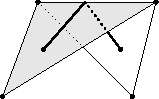
\includegraphics[width=0.9\linewidth]{figures/unfolding_geodesic.pdf}
      \caption{Folded in 3D space}
      \label{fig:geodesic-unfolding-folded}
    \end{subfigure}
    \hfill
    \begin{subfigure}[b]{0.49\linewidth}
      \centering
      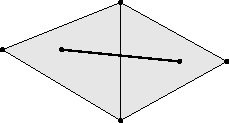
\includegraphics[width=\linewidth]{figures/unfolding_unfolded.pdf}
      \caption{Unfolded in 2D space}
      \label{fig:geodesic-unfolding-unfolded}
    \end{subfigure}
    \caption[Geodesic Unfolding of Two Adjacent Triangles]{%
      \textbf{Geodesic Unfolding of Two Adjacent Triangles}\\
      The figures visualize the geodesic unfolding process for two adjacent triangles with their common directed edge $e$ represented by its two vertices $v_1$ and $v_2$.
      The idea is to connect two given points $\tilde{p}$ and $\tilde{q}$ by a discrete geodesic that runs over $e$.
      To unfold the setting, $v_1$ is moved to center of the Euclidean plane and $e$ is mapped onto the $y$-axis.
    }
    \label{fig:geodesic-unfolding}
  \end{figure}

  Now, to calculate the intersection point in 2D, I will assume that $p_x < q_x$ which should be the case in general.
  Figure~\ref{fig:geodesic-unfolding-calculation} shows this calculation schematically.
  Again, the following notations will become useful later.
  \[
    \Delta x = q_x - p_x
    \separate
    \Delta y = q_y - p_y
    \separate
    \Sigma x = p_x + q_x
    \separate
    \Sigma y = p_y + q_y
  \]
  The straight line function $\function{f}{\setReal}{\setReal}$ connecting the two unfolded points looks like the following.
  \[
    f(x) = \frac{q_y - p_y}{q_x - p_x}(x - p_x) + p_y = \frac{q_y - p_y}{q_x - p_x}x + \frac{p_yq_x - q_yp_x}{q_x - p_x}
  \]
  Please note that this function is well-defined, as I assumed $q_x - p_x > 0$.
  To get the intersection point with the ordinate, the argument is set to zero.
  \[
    t\define f(0) = \frac{p_yq_x - q_yp_x}{q_x - p_x} = \frac{\Delta x \Sigma y - \Sigma x \Delta y}{2 \Delta x}
  \]

  \begin{figure}
    \centering
    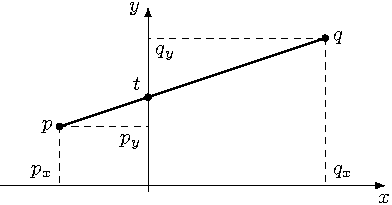
\includegraphics[width=0.6\linewidth]{figures/unfolding_geodesic_2d.pdf}
    \caption[Geodesic Unfolding Calculation Sketch]{%
      \textbf{Geodesic Unfolding Calculation Sketch}\\
      The sketch shows the meaning of variables for the unfolded step in the calculation of the geodesic unfolding primitive.
      The point $p$ is on the left side of the $y$-axis and the point $q$ on the right side.
      The goal is to connect both points by a straight line and compute the value $t$ that represents the intersection with the ordinate.
    }
    \label{fig:geodesic-unfolding-calculation}
  \end{figure}

  \noindent
  The last part of the calculation consists of scaling $t$ to fit the edge weight definition of λ.
  \[
    \tilde{λ} = \frac{t}{\norm{v_2-v_1}}
  \]
  It is important to note, that if $\tilde{λ}\not\in[0,1]$ then the points cannot be connected by a straightest geodesic that runs over the edge $e$.
  To handle the situation for the implementation of a smoothing primitive, the clamp method would be used.
  \[
    λ =
    \begin{cases}
      0 &: \tilde{λ} < 0 \\
      \tilde{λ} &: \tilde{λ}\in[0,1] \\
      1 & : \tilde{λ} > 1
    \end{cases}
  \]
  This will project the curve at this position onto one of the vertices of the common edge which would then be handled by another part of the algorithm.
  The following code snippet provides a straightforward implementation.

  \inputCodeBlock[title = Geodesic Unfolding]{code/geodesic-unfolding.hpp}

  \begin{lemma}[Geodesic Unfolding leads to Geodesics]
    Connecting $p$, $x$, and $q$ in that order by straight lines leads to locally shortest and straightest geodesics as long as $λ\in (0,1)$.
    It solves the discrete boundary value problem for locally shortest and straightest geodesics when boundary points lie in the interior of adjacent triangles.
  \end{lemma}
  % \begin{proof}
  %   According to \textcite{polthier2006} and \textcite{martinez2005}, locally shortest and straightest geodesics coincide on polyhedral if they do not contain any vertices.
  %   So, it is sufficient to show that the discrete curvature at the crease is zero.
  %   But this has be true by construction.
  % \end{proof}
  \noindent
  Please note, the geodesic unfolding is one of the two main operations \textcite{martinez2005} use to iteratively transform an initially given surface mesh curve into a locally shortest geodesic.


  \paragraph{Curvature-Based Unfolding of Two Adjacent Triangles}\hfill\\
    Assume the same setting as in the previous part about the geodesic unfolding of two adjacent triangles.
    The curvature-based unfolding primitive does not try to find a geodesic in $S$ connecting the points $\tilde{p}$ and $\tilde{q}$.
    Instead, its goal is to find a point $x_κ \in e$ with its edge weight $λ_κ\in[0,1]$ for an angle $κ\in(-π,π)$ such that the discrete geodesic curvature at $x_κ$ of the curve segment, given by the straight-line connection of $p$, $x_κ$, and $q$, coincides with the value of $κ$.
    \[
      x_κ = (1-λ_κ)v_1 + λ_κ v_2
    \]
    Using the same unfolding mechanism and notation as before, this setting is schematically visualized by figure~\ref{fig:curvature-unfolding} for positive and negative values of κ.
    For $κ=0$, this primitive reduces to the previous case of geodesic unfolding.

    \begin{figure}
      \centering
      \begin{subfigure}[b]{0.49\linewidth}
        \centering
        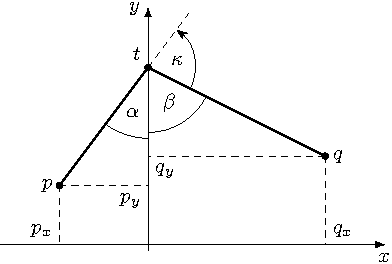
\includegraphics[width=\linewidth]{figures/unfolding_curvature_2d.pdf}
        \caption{$κ < 0$}
      \end{subfigure}
      \hfill
      \begin{subfigure}[b]{0.49\linewidth}
        \centering
        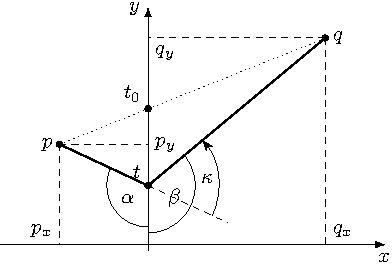
\includegraphics[width=\linewidth]{figures/unfolding_curvature_2d_positive.pdf}
        \caption{$κ > 0$}
      \end{subfigure}
      \caption[Curvature-Based Unfolding Calculation Sketch]{%
        \textbf{Curvature-Based Unfolding Calculation Sketch}\\
        The sketches show the meaning of variables for the unfolded step in the calculation of the curvature-based unfolding primitive for positive and negative geodesic curvatures.
        The point $p$ is on the left side of the $y$-axis and the point $q$ on the right side.
        The goal is to find $t$ such that the line segments from $p$ over $(0,t)$ to $q$ exhibit a discrete geodesic curvature of $κ$ at $(0,t)$.
      }
      \label{fig:curvature-unfolding}
    \end{figure}

  As the derivation of this primitive is a little bit more involved,
  % I will show the calculations only for $κ > 0$ and
  I will start with an observation for both sides individually.
  For this, I again assume $p_x < 0$ and $q_x > 0$.
  As given in figure~\ref{fig:curvature-unfolding}, let $α,β\in(0,π)$ and $κ\in(-π,π)$ with $κ < α$ and $π+κ > α$.
  Using the appropriate sign for κ, the following is always true.
  \[
    κ + π = α + β
  \]
  Now, the functions $f$ and $g$ of line segments, that connect $p$ with $(0,t)$ and $(0,t)$ with $q$, respectively, are given as follows.
  \[
    f(x) = p_y + (x - p_x)\cot α
    \separate
    g(x) = q_y - (x - q_x)\cot β
  \]
  Their value for the intersection with the ordinate can directly be inferred.
  \[
    f(0) = p_y - p_x \cot α
    \separate
    g(0) = q_y + q_x \cot β
  \]
  After the individual inspection of both sides, the following equation results from the equation $f(0)=t=g(0)$ that stems from the fact that both values at the ordinate need to coincide.
  \[
    p_y - p_x \cot α = q_y + q_x \cot β
  \]
  To solve this equation, I will express $\cot β$ with the use of $\cot α$ and κ and by the application of a trigonometric identity for the cotangent.
  \[
    \cot β = \cot(π-(α-κ)) = -\cot(α-κ) = - \frac{\cos κ \cot α + \sin κ}{\cos κ - \sin κ \cot α}
  \]
  % \[
  %   \cot(α-κ) = \frac{\cot α \cot κ + 1}{\cot κ - \cot α}
  % \]
  % \[
  %   p_y - p_x \cot α = q_y - q_x \frac{\cot α \cot κ + 1}{\cot κ - \cot α}
  % \]
  To shorten the notation, redefine $\cot α$ to be the variable that needs to be computed and insert everything into the main equation.
  \[
    φ\define \cot{α}
    \separate
    % K\define \cot κ
    p_y - p_x φ = q_y - q_x \frac{φ \cos κ + \sin κ}{\cos κ - φ \sin κ}
  \]
  Put the fraction on the left side of the equation.
  \[
    q_x \frac{φ \cos κ + \sin κ}{\cos κ - φ \sin κ} = q_y - p_y + p_x φ
  \]
  Multiply both sides with the denominator.
  \[
    φ q_x \cos κ + q_x \sin κ
    = (\Delta y + φ p_x)(\cos κ - φ \sin κ)
  \]
  And expand the resulting equation as follows.
  \[
    φ q_x \cos κ + q_x \sin κ
    = \Delta y \cos κ - φ \Delta y \sin κ + φ p_x \cos κ - φ^2 p_x \sin κ
  \]
  Put it now into the form of a quadratic equation.
  \[
    φ^2 p_x \sin κ + φ (\Delta x \cos κ + \Delta y \sin κ) + q_x \sin κ - \Delta y \cos κ = 0
  \]
  The solution to this quadratic equation is given by the following expression.
  \[
    \begin{aligned}[t]
      φ = \frac{1}{2 p_x \sin κ} \bigg[
      &-(\Delta x \cos κ + \Delta y \sin κ) \\
      &\pm \sqrt{(\Delta x \cos κ + \Delta y \sin κ)^2 - 4p_x \sin κ (q_x \sin κ - \Delta y \cos κ)} \bigg]
    \end{aligned}
  \]
  Simplify the expression inside the square root.
  \[
    φ = \frac{1}{2 p_x \sin κ} \boxBrackets{-(\Delta x \cos κ + \Delta y \sin κ) \pm \sqrt{(\Sigma x \cos κ + \Delta y \sin κ)^2 - 4 p_x q_x}}
  \]
  Now, insert the equation for φ given above into $t = f(0) = p_y - p_x φ$ and get the following.
  \[
    t = \frac{1}{2 \sin κ} \boxBrackets{\Delta x \cos κ + \Sigma y \sin κ \pm \sqrt{(\Sigma x \cos κ + \Delta y \sin κ)^2 - 4 p_x q_x}}
  \]
  To get the difference to the previous unfolding primitive and being able to cope with the $κ=0$ singularity, let $t_0$ be the intersection value of the straight line connecting $p$ and $q$ with the $y$-axis and define $\Delta t \define t - t_0$ as the difference of the previous and the current primitive.
  Put $t_0$ inside the expression for $t$ by adding zero.
  \[
    t = t_0 + \frac{1}{2 \sin κ} \boxBrackets{-2t_0\sin κ + \Delta x \cos κ + \Sigma y \sin κ \pm \sqrt{(\Sigma x \cos κ + \Delta y \sin κ)^2 - 4 p_x q_x}}
  \]
  Use the expression for $t_0$ from previous part about geodesic unfolding.
  \[
    t_0 = \frac{1}{2}\roundBrackets{\Sigma y - \Sigma x \frac{\Delta y}{\Delta x}}
  \]
  Put the expression for $t_0$ into the previous equation and deduce the expression $\Delta t$.
  \[
    \Delta t = \frac{1}{2 \sin κ} \boxBrackets{\Sigma x \frac{\Delta y}{\Delta x}\sin κ + \Delta x \cos κ \pm \sqrt{(\Sigma x \cos κ + \Delta y \sin κ)^2 - 4 p_x q_x}}
  \]
  For this expression, there is only one valid sign as $2 \Delta t \sin κ \leq 0$ must hold.
  % Consequently, the following expression is the true solution.
  % \[
  %   2 \Delta t \sin κ \leq 0
  % \]
  \[
    \Delta t = \frac{1}{2 \sin κ} \boxBrackets{\Sigma x \frac{\Delta y}{\Delta x}\sin κ + \Delta x \cos κ - \sqrt{(\Sigma x \cos κ + \Delta y \sin κ)^2 - 4 p_x q_x}}
  \]
  If $κ=0$ then $t$ or $\Delta t$ would be undefined.
  However, the expression for $\Delta t$ can simply be set to zero as $t_0$ is the correct solution in that case.
  Similarly to the previous part, $\Delta t$ needs to be scaled to fit the definition of the edge weight.
  \[
    \tilde{λ}_κ \define \frac{t_0 + \Delta t}{\norm{v_2-v_1}} = \tilde{λ} + \frac{\Delta t}{\norm{v_2-v_1}}
  \]
  Again, we cannot find a valid point on the edge $e$ that fulfills the constraint, if $\tilde{λ}_κ\not\in[0,1]$.
  Therefore the clamp routine is used again.
  \[
    λ_κ =
    \begin{cases}
      0 &: \tilde{λ}_κ < 0 \\
      \tilde{λ}_κ &: \tilde{λ}_κ\in[0,1] \\
      1 & : \tilde{λ}_κ > 1
    \end{cases}
  \]
  Please note, this curvature-based unfolding of two adjacent triangles is very similar to the primitive used by \textcite{lawonn2014} to iteratively smooth surface mesh curves based on desired geodesic curvatures.
  But \citeauthor{lawonn2014} derive their equation by using a different strategy with an non-oriented geodesic curvature which leads to an alternative formulation that could lead to numerical instabilities.
  I have carried out the derivation of the above primitive to provide a single formulation for all values of the oriented discrete geodesic curvature that is able to handle the $κ=0$ singularity.
  The following code snippet provides a straightforward implementation.

  \inputCodeBlock[title = Curvature-Based Unfolding]{code/curvature-unfolding.hpp}

  \paragraph{Local Smoothing}\hfill\\
  With the smoothing primitives in place, it is now possible to define the local smoothing procedure for a surface mesh curve.
  The essential part of this routine is to iterate over the control points that lie in the curve's interior and apply one of the two unfolding primitives given above.
  For that, each interior control point accesses the previous and next control point of the curve.
  For closed curves, all control points are part of the interior and the first and last one coincide.
  To updated a closed curve accordingly, let the first control point access the one before the last and also apply the unfolding primitive.
  The underlying topology of the surface mesh curve given in the form of an edge sequence or face strip is not altered.
  The following code snippet shows a simple implementation of this strategy for the face-based data structure.
  The implementation for the edge-based structure is omitted because the retrieval of edge vertices and control points is only a subset of the face-based code.

  \inputCodeBlock[title = Local Smoothing]{code/local-smoothing.hpp}
  There is nothing special happening in the code above apart from the retrieval of edge vertices by using face nodes.
  The face nodes of the face-based data structure use their \textbf{\texttt{loc}} and \textbf{\texttt{rot}} members to point to the edges of the previous and next adjacency edge.
  The next directed edge that points to the right side cannot be part of the oriented triangle that describes the face.
  Hence, its indices are exchanged to properly retrieve the next directed edge.

  Another remark is that the code for the whole update iteration uses the old edge weights of the curve.
  In a serial implementation that needs to converge fast, an in-place update of all the edge weights could be used instead of swapping all newly created edge weights with the old ones at end of the procedure.
  In this scenario, all edge weights apart from the first one would use an updated control point on their left side.
  In fact, this method has been used by \textcite{martinez2005} and \textcite{lawonn2014} and may lead to a faster convergence.
  On the other hand, all the outcomes before reaching a certain convergence tend to exhibit asymmetric changes in the curvature of the surface mesh curve.
  As for smoothing, algorithms may also be aborted without any convergence because the outcome is already smooth enough.
  By using the swapping mechanism, I make sure all applications of the local smoothing provide a consistent and symmetric smoothing.

  \paragraph{Unfolding of Triangle Fans around a Reflex Vertex}\hfill\\
  Besides the unfolding of two adjacent triangles, the reflection procedure will also need a primitive which is able to unfold a whole strip of triangles that share a common vertex.
  As soon as the reflection will move the topology of a curve to the other side of a reflex vertex, all weights for the new edges on the opposite triangle fan need to be assigned.
  This can be seen in figure~\ref{fig:local-reflection}.
  % Referring to the turn compression scheme, the triangles all describe the same turn.
  The goal is to connect the previous point $p$ with the next point $q$ either by a geodesic, as in the geodesic unfolding primitive, or by a surface mesh curve with the desired geodesic curvatures as in the case of the curvature-based unfolding primitive.
  Therefore it is not possible to independently assign weights to the edges between the points $p$ and $q$.
  Figure~\ref{fig:unfolding-critical-vertex} schematically visualizes this scenario.

  \begin{figure}
    \centering
    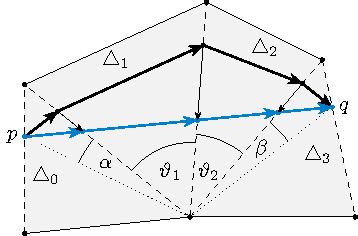
\includegraphics[width=0.55\linewidth]{figures/unfolding-critical-vertex.pdf}
    \caption[Unfolding of a Triangle Fan around a Reflex Vertex]{%
      \textbf{Unfolding of a Triangle Fan around a Reflex Vertex}\\
      The scheme illustrates the unfolded triangle fan around a reflex vertex $v_0$ and surface mesh curve given as thick, black line.
      The blue line represents the resulting surface mesh curve after the application of the triangle fan unfolding primitive and connects the previous point $p$ and the next point $q$ by a straight line in the unfolding plane.
    }
    \label{fig:unfolding-critical-vertex}
  \end{figure}

  Let both the previous point $p$ and the next point $q$ be given relative to the inner vertex $v_0$.
  Furthermore, for $n\in\setNatural$, let $v_1,\ldots,v_n\in \mathscr{S}$ be the outer vertices of the common edges of the triangle strip that shares $v_0$.
  Define the edge vectors as follows.
  \[
    e_i \define \frac{v_i-v_0}{\norm{v_i-v_0}}
  \]
  All triangles need to be unfolded in the 2D Euclidean plane as it was already done in the case of the geodesic unfolding.
  The only difference is that this time more than two triangles need to be unfolded.
  Therefore I start with the points $p$ and $q$.
  \[
    p_x^1 \define \scalarProduct{p}{e_1}
    \separate
    p_y^1 \define \norm{p - p_x^1 e_1}
    \separate
    q_x^n \define \scalarProduct{q}{e_n}
    \separate
    q_y^n \define -\norm{q - q_x^n e_n}
  \]
  To get back to the previous cases, the point $p$ must be transformed into the coordinate system of $q$ whose $y$-axis is given by the edge $e_n$.
  As the triangles are folded in 3D space, this needs to be done iteratively for the whole triangle fan.
  Inside of a triangle, transforming one edge coordinate system to the other can be done by using an orthogonal 2D rotation matrix.
  \[
    \cos ϑ_i = \scalarProduct{e_i}{e_{i+1}}
    \separate
    \sin ϑ_i = \norm{e_i - e_{i+1} \cos ϑ_i}
  \]
  \[
    R_i \define
    \begin{pmatrix}
      \cos ϑ_i & -\sin ϑ_i \\
      \sin ϑ_i & \cos ϑ_i
    \end{pmatrix}
    \separate
    R_i^{-1} = R_i^\mathrm{T}
  \]
  The last part then consists of using the rotation matrices to transform the coordinate representations of the points $p$ and $q$ to all edges.
  \[
    \begin{pmatrix}
      p_x^{i+1} \\
      p_y^{i+1}
    \end{pmatrix}
    = R_i
    \begin{pmatrix}
      p_x^{i} \\
      p_y^i
    \end{pmatrix}
    \separate
    \begin{pmatrix}
      q_x^{i} \\
      q_y^{i}
    \end{pmatrix}
    = R^{-1}_i
    \begin{pmatrix}
      q_x^{i+1} \\
      q_y^{i+1}
    \end{pmatrix}
  \]
  In such a way, all the unfolded $x$ and $y$ coordinates of $p$ and $q$ can be computed for every edge.
  The geodesic unfolding can then again simply applied to every edge independently to determine the edge weights of the geodesic connecting $p$ and $q$.

  To determine edge weights with the correct geodesic curvature, a slight change needs to be introduced.
  As the curvature-based primitive is not linearly dependent of its adjacent control points, like in the case of the geodesic unfolding, the edge weights cannot be evaluated independently even after the transformation of coordinate representations.
  % Furthermore, the desired curvatures for all edges need to be the same.
  Instead, the right-most edge can be evaluated first.
  Hereby, the desired curvature for the unfolding will be given by the sum of all desired curvatures.
  After the unfolding step, the desired curvature for the next unfolding will be the current one reduced by the desired curvature of the current edge.
  All other edges will then be done iteratively in the same way with an alternated point $\tilde{q}$ to the right that is given by the result of the previous edge computation.
  This is the same process as given by \textcite{lawonn2014}.


  \paragraph{Reflection}\hfill\\
  The local reflection primitive retrieves the reflected topology at a reflex vertex.
  For that, assume that the turn compression of the surface mesh curve has already been computed and is available for use.
  A reflection can only be applied to a compressed turn node as I expect the first and the last triangle given for the reflection to exhibit an edge rotation that is opposite to the triangle fan which in figure~\ref{fig:local-reflection} is illustrated.
  The reflection primitive returns a new temporary face strip for the current turn of the curve.
  For the example in figure~\ref{fig:local-reflection}, it would look like the following.
  \[
    (\triangle_p,\triangle_1,\triangle_2,\triangle_3,\triangle_4,\triangle_q)
    \separate
    \longrightarrow
    \separate
    (\triangle_p,\tilde{\triangle}_1,\triangle_q)
  \]
  By applying the previous unfolding primitive for triangle fans, the new weights of the common edges of the new triangle strip can be evaluated.
  After the computation, triangle strip and edge weights may be exchanged with the old triangle fan and its edge weights.
  Please note, for reflex vertices that are part of the boundary, no reflected path exists.

  \begin{figure}
    \centering
    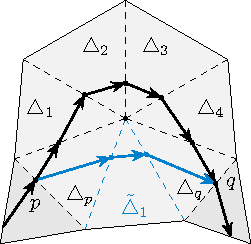
\includegraphics[width=0.45\linewidth]{figures/local-reflection.pdf}
    \caption[Local Reflection at a Reflex Vertex]{%
      \textbf{Local Reflection at a Reflex Vertex}\\
      The image illustrates how the face strip of a surface mesh curve, shown as thick and black line, changes when the local reflection primitive is applied.
      Its result is given by the blue line.
    }
    \label{fig:local-reflection}
  \end{figure}

  \inputCodeBlock[title = Local Reflection]{code/local-reflection.hpp}
  The code above implements the local reflection for the face-based data structure with the use of the generated face adjacency structure.
  Conveniently, this routine deals with self-intersections of surface mesh curves that get to small by removing them.
  In this case, when exchanging the old triangle strip with the reflected one, care needs to be taken as the the transformed surface mesh curve may violate the regularity condition.
  It is important to remove triangles that are doubled or returning to the previous one.
  This primitive is a major deviation from the design shown by \textcite{lawonn2014} because no projections of control points to vertices of the surfaces are used.
  Instead, it complies with a method described by \textcite{mancinelli2022}.

  \paragraph{Algorithm}\hfill\\
  After the definition of all primitives, the main smoothing algorithm mainly uses the

  The main algorithm only switches between reflection and local smoothing.
  The abort criterion was chosen in the same way as lawonn and martinez.

  For open curves, iterate through the turn compression and apply unfolding of triangle fans.
  For closed curves, ignore the first turn as it might also contain turns from the end.
  When reaching the end, check whether the first turn belongs to the last.

  Each turn unfolding might lead to a critical vertex.
  Mark the turn.
  After applying turn unfolding, check for marked vertices

  As we are constantly changing the number of control points of triangles in the face strip, a queue-based approach seems to be most fitting.

  \paragraph{Smoothing via Desired Geodesic Curvatures}\hfill\\
  I introduce the desired curvature stencil.
  This allows to smooth such that they keep very close to their original form.

  \inputCodeBlock[title = Desired Curvature Stencil]{code/desired-curvature-stencil.hpp}


% subsection smoothing_of_surface_mesh_curves (end)

% \subsection{Overview of the Program Pipeline} % (fold)
% \label{sub:program_pipeline}
%   In the following, the stages of the implemented program pipeline are stated and summarized.
%   These stages naturally arise from an insight into the generation and tracing of geodesics on surface meshes, described in section~\ref{sec:previous_work}.
%   Locally shortest or straightest geodesics that follow as a solution from the discrete boundary value problem are in some sense the smoothest curves that cannot be made any smoother.
%   As we typically need to provide an initial curve for those geodesics to be found, the whole generation and tracing of geodesics can be looked at as an extreme smoothing process.
%   Adding parameters to let the user decide on when to stop this process then results in the pipeline given below and schematically shown in figure~\ref{fig:program-pipeline}.

%   \begin{figure}[h]
%     \begin{center}
%       \large
%       INSERT YOUR IMAGE HERE!
%     \end{center}
%     \caption[Program Pipeline Stages]{%
%       \textbf{Program Pipeline Stages}\\
%       The scheme shows all the stages of the implemented program pipeline.
%       The arrows indicate data flow and dependencies.
%     }
%     \label{fig:program-pipeline}
%   \end{figure}

%   \begin{enumerate}
%     \item \textbf{Surface Mesh Loading:}\\
%       Load a surface mesh given by a specific file format from the storage.
%     \item \textbf{Surface Mesh Preprocessing:}
%       \begin{enumerate}
%         \item Generate a connected mesh object to properly model the topology of the input.
%         \item Generate the pseudo-normals for each vertex.
%         \item Generate the dual graph for the neighbors of each triangle.
%         \item Check that the mesh is a valid orientable two-dimensional topological manifold.
%       \end{enumerate}
%     \item \textbf{Initial Curve Selection:} \\
%       Let the user choose an initial curve by drawing on the surface.
%     \item \textbf{Parameter Selection:} \\
%       Let the user choose parameters for the curve smoothing algorithm.
%     \item \textbf{Curve Smoothing:} \\
%       Smooth the initial curve according to the constraints given by the selected parameters.
%     \item \textbf{Postprocessing:} \\
%       Optionally apply the smoothed curve in a domain-specific context.
%   \end{enumerate}
%   According to figure~\ref{fig:program-pipeline}, the output of every stage is not only forwarded to the next stage but also specifically visualized and rendered to the screen to provide the user with visual feedback and to catch errors or exceptional behavior as early as possible.
%   Besides, additional user interactions will be processed for all stages to allow for measurements and adjustments and to be able to react to the output of previous stages.
%   The loading of surface meshes from different file formats is typically handled by loader libraries, such as \textit{Assimp}, and will not be further explained.
%   On the other hand, surface mesh preprocessing and the initial curve selection are crucial steps in the whole pipeline which remove geometric degeneracies and artifacts that would otherwise violate assertions needed for the correct execution of the algorithm.
%   Therefore both stages will be discussed in more detail in the following subsections.
%   The postprocessing in our case is optional and only provided for the sake of completeness.
%   The parameter selection is highly dependent on the implementation of the curve smoothing algorithm and, as a result, it will be described together with the curve smoothing itself.
% % subsection program_pipeline (end)

% \subsection{Surface Mesh Preprocessing} % (fold)
% \label{sub:mesh_preprocessing}
%   The goal of preprocessing a surface mesh which has been loaded from disk is to transform its data into a valid and efficient representation of a polyhedral surface that should exhibit functionality to draw and move points and discrete curves on its surface.
%   In the case that this transformation is not possible, the stage at least must check for the validity of the given data and emit an error if there might be any violations.
%   % On one hand, the preprocessing of a given surface mesh needs to make sure that the program or algorithm is actually dealing with a valid two-dimensional topological manifold.

%   A given Mesh for the algorithm can be quite general.
%   Providing triangles which will introduce numerical difficulties is out of the scope of this thesis.

%   We will focus on orientable meshes.
%   Please note, that is not an actual restriction for the algorithm but will only speed up the implementation.
%   Furthermore, we look at surfaces which are the boundary of volumes in three-dimensional Euclidean space which can be looked at as open submanifolds.
%   These volumes are therefore by definition oriented and, hence, their boundary needs to be, too.
%   Still, we need to look boundaries for surfaces as, for example, distance envelopes restrict the surface without boundary to be one.
%   The boundaries need to be handled properly.
%   Also, these requirements are only need to hold for the restriction to the distance envelope.
%   Often, lines will be drawn on oriented/orientable parts of the surface even if the surface is not orientable due to artifacts originating from scanning or generating meshes.

%   \paragraph{Topological Connections}
%   We need the topological connections of a given surface mesh.
%   In the case of general file formats, a scene is typically separated into multiple meshes which are topologically but not smoothly connected.
%   For proper drawing of curves in a whole scene, the topological structure of connections needs to be generated first.
%   Using the STL file format, this is not needed.

%   \paragraph{Generating the dual graph}
%    To generate such a dual graph we refer to this book.
%   It is assumed to be a solved problem.
%   First, we have created a hash map of oriented edges with a custom hash function to mangle vertex indices.
%   The mapped values store the faces indices and their location in the triangle.
%   By inverting the indices of a stored edge, one can easily access the neighboring triangle if it exists.
%   Furthermore, it is easy to check whether the mesh is oriented and a valid two-dimensional manifold.

%   \paragraph{Check for orientability and validity}

% % subsection mesh_preprocessing (end)

% \subsection{Initial Curve Selection} % (fold)
% \label{sub:initial_curve_selection}
%   As for the vast majority of optimization algorithms, the results and efficient working are highly dependent on the chosen starting values.
%   Curve smoothing itself is an optimization process and to solve the boundary value problem, we need an initial value.
%   So, choosing the initial curve in the right way will also heavily change the speed and quality of the algorithm.
%   The algorithm should be able to handle a vast amount unsmooth curves.
%   Still, the handling of artifacts will be taken care of at the start.
%   \paragraph{User Interface for Selecting and Controlling Initial Curves}
%   \paragraph{Drawing by Ray Tracing}
%   \paragraph{Connecting the Vertices}
%   \paragraph{Closed Initial Curves and Fixed Vertices}
%   \paragraph{Artifact Removal}
%   \paragraph{Smoothed Curvature Values by Stencil}
%     Stencil is discrete approximation of solution to Laplacian equation or heat equation which is smooth (infinitely differentiable).
%     Maybe it would be useful to keep the length of the curve and still smooth it.
%   \paragraph{Vertex Curves}
%   \paragraph{Face Curves}
%   \paragraph{Tracing Geodesics}
% % subsection initial_curve_selection (end)



%   \begin{figure}[h]
%     \centering
%     \begin{subfigure}[b]{0.49\linewidth}
%       \centering
%       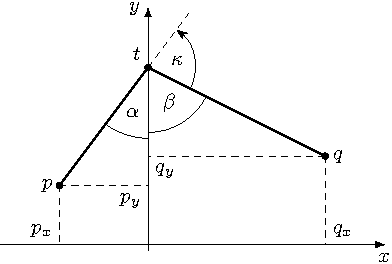
\includegraphics[width=\linewidth]{figures/unfolding_curvature_2d.pdf}
%       \caption{$κ < 0$}
%     \end{subfigure}
%     \hfill
%     \begin{subfigure}[b]{0.49\linewidth}
%       \centering
%       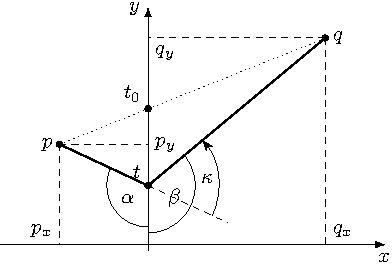
\includegraphics[width=\linewidth]{figures/unfolding_curvature_2d_positive.pdf}
%       \caption{$κ > 0$}
%     \end{subfigure}
%     \caption[2D Unfolding Curvature Primitive]{%
%       \textbf{2D Unfolding Curvature Primitive}\\
%     }
%     \label{fig:}
%   \end{figure}

% Again, a two-dimensional primitive is used.
% \[
%   f(x) = -\cot α (x - p_x) + p_y
% \]
% \[
%   t = f(0) = p_y + \absolute{p_x}\cot α
% \]
% Now, combine two points to both sides with a desired discrete curvature.
% For this, assume $p_x < 0$ and $q_x > 0$.
% Furthermore, the desired curvature is positive $κ > 0$ and taken mathematically positive.
% $α,β\in(0,π)$ and $κ\in(-π,π)$ with $κ < α$ and $π+κ > α$
% \[
%   κ + π = α + β
% \]
% From the former computation, it is clear that their points on the ordinate have to coincide.
% \[
%   p_y - p_x \cot α = q_y + q_x \cot β
% \]
% \[
%   \cot β = \cot(π-(α-κ)) = -\cot(α-κ)
% \]
% \[
%   \cot(α-κ) = \frac{\cos κ \cot α + \sin κ}{\cos κ - \sin κ \cot α}
% \]
% % \[
% %   \cot(α-κ) = \frac{\cot α \cot κ + 1}{\cot κ - \cot α}
% % \]
% % \[
% %   p_y - p_x \cot α = q_y - q_x \frac{\cot α \cot κ + 1}{\cot κ - \cot α}
% % \]
% \[
%   φ\define \cot{α}
%   % \separate
%   % K\define \cot κ
% \]
% \[
%   p_y - p_x φ = q_y - q_x \frac{φ \cos κ + \sin κ}{\cos κ - φ \sin κ}
% \]
% \[
%   q_x \frac{φ \cos κ + \sin κ}{\cos κ - φ \sin κ} = q_y - p_y + p_x φ
% \]
% \[
%   φ q_x \cos κ + q_x \sin κ
%   = (\Delta y + φ p_x)(\cos κ - φ \sin κ)
% \]
% \[
%   φ q_x \cos κ + q_x \sin κ
%   = \Delta y \cos κ - φ \Delta y \sin κ + φ p_x \cos κ - φ^2 p_x \sin κ
% \]
% \[
%   φ^2 p_x \sin κ + φ (\Delta x \cos κ + \Delta y \sin κ) + q_x \sin κ - \Delta y \cos κ = 0
% \]
% \[
%   φ = \frac{1}{2 p_x \sin κ} \boxBrackets{-(\Delta x \cos κ + \Delta y \sin κ) \pm \sqrt{(\Delta x \cos κ + \Delta y \sin κ)^2 - 4p_x \sin κ (q_x \sin κ - \Delta y \cos κ)}}
% \]
% \[
%   φ = \frac{1}{2 p_x \sin κ} \boxBrackets{-(\Delta x \cos κ + \Delta y \sin κ) \pm \sqrt{(\Sigma x \cos κ + \Delta y \sin κ)^2 - 4 p_x q_x}}
% \]
% \[
%   t = \frac{1}{2 \sin κ} \boxBrackets{\Delta x \cos κ + \Sigma y \sin κ \pm \sqrt{(\Sigma x \cos κ + \Delta y \sin κ)^2 - 4 p_x q_x}}
% \]
% \[
%   t = t_0 + \Delta t
% \]
% \[
%   t = t_0 + \frac{1}{2 \sin κ} \boxBrackets{-2t_0\sin κ + \Delta x \cos κ + \Sigma y \sin κ \pm \sqrt{(\Sigma x \cos κ + \Delta y \sin κ)^2 - 4 p_x q_x}}
% \]
% \[
%   t_0 = \frac{1}{2}(\Sigma y - \Sigma x \frac{\Delta y}{\Delta x})
% \]
% \[
%   \Delta t = \frac{1}{2 \sin κ} \boxBrackets{\Sigma x \frac{\Delta y}{\Delta x}\sin κ + \Delta x \cos κ \pm \sqrt{(\Sigma x \cos κ + \Delta y \sin κ)^2 - 4 p_x q_x}}
% \]
% \[
%   2 \Delta t \sin κ \leq 0
% \]
% \[
%   \Delta t = \frac{1}{2 \sin κ} \boxBrackets{\Sigma x \frac{\Delta y}{\Delta x}\sin κ + \Delta x \cos κ - \sqrt{(\Sigma x \cos κ + \Delta y \sin κ)^2 - 4 p_x q_x}}
% \]
% \[
%   Kq_xφ + q_x = \Delta y φ - K\Delta y + p_x φ^2 - Kp_x φ
% \]
% \[
%   q_x + K\Delta y = p_x φ^2 + (\Delta y -K(p_x+q_x))φ
% \]
% \[
%   \frac{q_x + K\Delta y}{p_x} = φ^2 + \frac{\Delta y - K\Sigma x}{p_x}φ
% \]
% \[
%   φ = -\frac{\Delta y - K\Sigma x}{2p_x} \pm \sqrt{\frac{q_x + K\Delta y}{p_x} + \frac{(\Delta y - K\Sigma x)^2}{4p^2_x}}
% \]
% \[
%   t = p_y - p_x φ
% \]
% \[
%   t = p_y + \frac{\Delta y - K\Sigma x}{2} \mp \sqrt{p_x(q_x + K\Delta y) + \frac{(\Delta y - K\Sigma x)^2}{4}}
% \]
% \[
%   t = \frac{\Sigma y - K\Sigma x}{2} \mp \sqrt{p_x(q_x + K\Delta y) + \frac{\Delta^2y - 2K\Delta y\Sigma x + K^2\Sigma^2x}{4}}
% \]
% \[
%   t = \frac{\Sigma y - K\Sigma x}{2} \mp \sqrt{p_xq_x(1 + K^2) + \frac{\Delta^2y - 2K\Delta y\Delta x + K^2\Delta^2x}{4}}
% \]
% \[
%   t = \frac{\Sigma y - K\Sigma x}{2} \mp \sqrt{p_xq_x(1 + K^2) + \frac{(\Delta y - K\Delta x)^2}{4}}
% \]
% subsection unfolding_with_desired_curvature (end)

% \subsection{Desired Curvature Stencil} % (fold)
% \label{sub:desired_curvature_stencil}

% % subsection desired_curvature_stencil (end)

% \subsection{Desired Curvature Mapping} % (fold)
% \label{sub:desired_curvature_mapping}

% % subsection desired_curvature_mapping (end)

% \subsection{Curve Smoothing Algorithm} % (fold)
% \label{sub:curve_smoothing_algorithm}
%   Curve smoothing is not a discrete problem.
%   Using only a finite amount of steps is probably not possible.
%   So, we use a process of convergence.
%   This has the advantage that not all triangles need to be unfolded at once.
%   This makes the implementation and parallelization much simpler.
%   The discrete algorithms for tracing geodesics are not easy to parallelize.

%   \paragraph{Idea and Overview}
%   \paragraph{Edge Vertex Relaxation}
%     We need to take a look at topological and numerical robustness.
%   \paragraph{Vertex Vertex Relaxation}
%   \paragraph{Critical Vertex Handling}
%   \paragraph{Artifact Removal and Self-Intersection Handling}
%   \paragraph{Desired Curvature Mapping}
%     Desired curvatures need to be constant along edges.
%     Therefore interpolate on angle-basis around vertex.
%     We do not want to loose information of desired curvatures.
%   \paragraph{Curve Evaluation}
%   \paragraph{Correctness and Convergence}
%     Correctness can be shown by showing the convergence to the curvature values.
%     This by definition of the given curvature values smooths the curve.
%     The convergence might only be shown for contracting the curve by smoothing.
%     As the limit is the geodesic, the prove of its convergence is there.
%   \paragraph{Complexity}
% % subsection curve_smoothing_algorithm (end)

% section design (end)
\end{document}
